
\section{Results}

??? screenshots of spatial patterns ???


\subsection{Effect of spatial structure in PD and HD games}

In our first simulation experiment, we compared the effect of spatial structure on the persistence of cooperators in the PD and HD games.


(figure \ref{fig: task1_4plot})



\begin{figure}[H]
	\centering 
	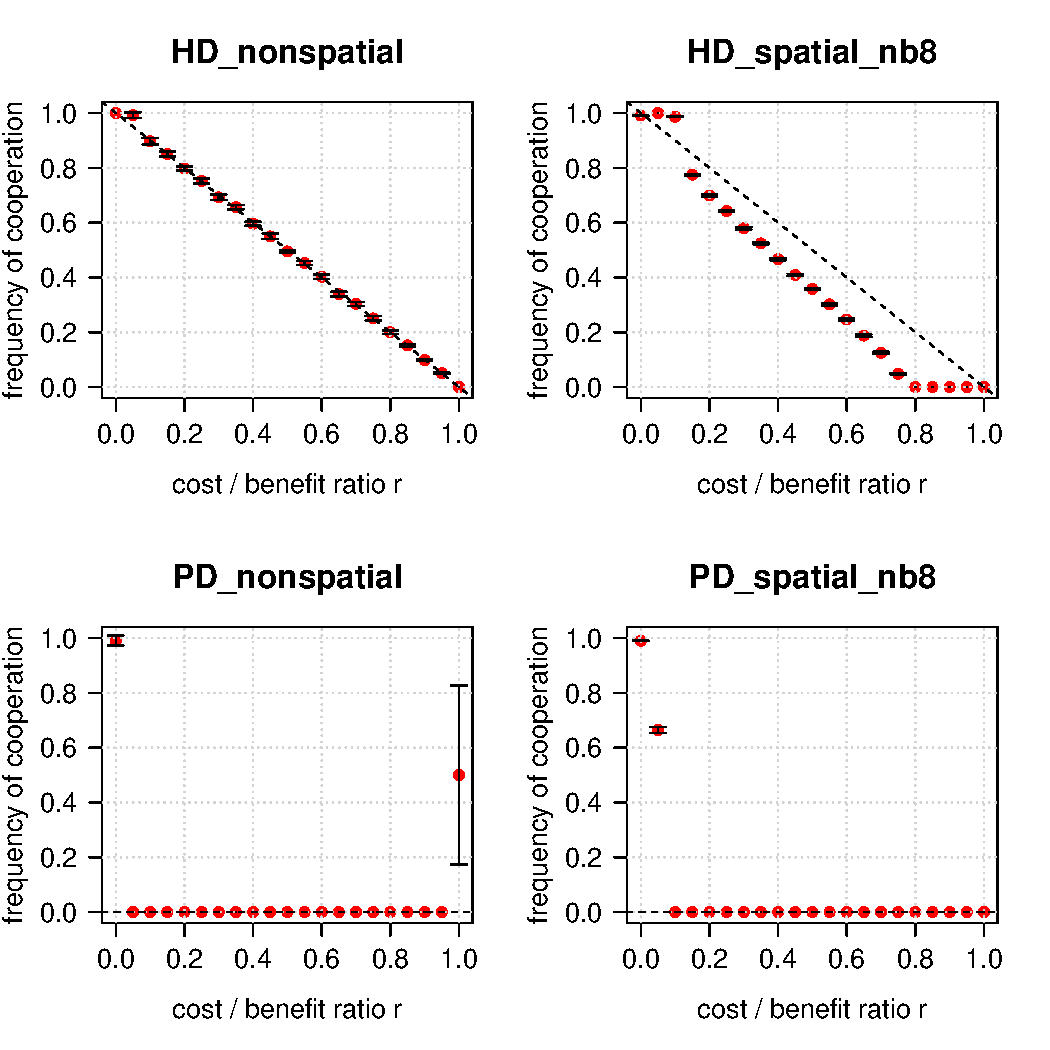
\includegraphics[width=9.5cm]{task1_4plot}
	\caption{Comparison of HD and PD game simulations, both with and without spatial structure.  \textbf{[ t = 5000, i = 10 ]} }\label{fig: task1_4plot}
\end{figure}






\subsection{Effect of neighbourhood size}

In the second simulation experiment we investigated the effect of 

\textbf{HD games}

\begin{figure}[H]
	\centering 
	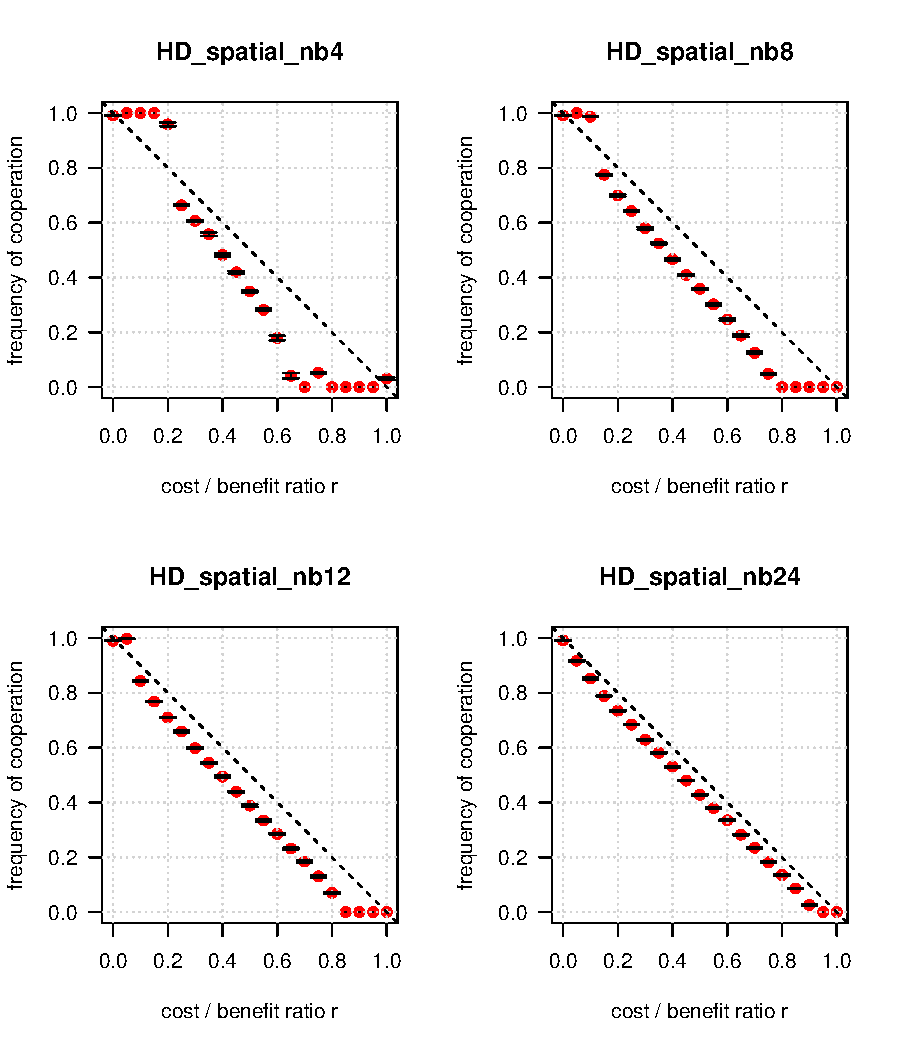
\includegraphics[width=9.5cm]{task2_4plot}
	\caption{Effect of varying neighborhood size in the HD game.  \textbf{[ t = 5000, i = 10 ]} }\label{fig: task2_4plot}
\end{figure}



\textbf{PD games} 


\begin{figure}[H]
	\centering 
	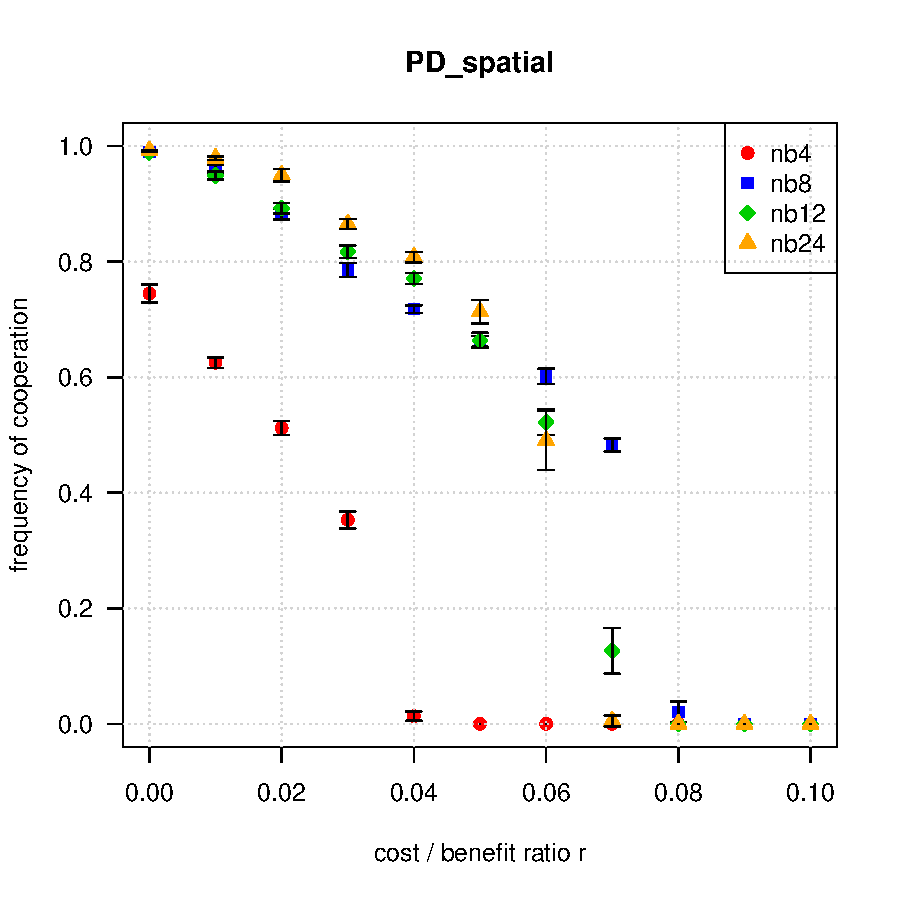
\includegraphics[width=9.5cm]{task2_multiplot}
	\caption{Spatial PD game simulations with different neighborhood sizes.  \textbf{[ t = 5000, i = 10 ]} }\label{fig: task2_multiplot}
\end{figure}


It is widely assumed that spatial structure allows for the evolution of cooperation in PD games. However, this goes only for a small range of cost-benefit ratios. Cooperation is only evolutionarily stable for r-values $ \leq 0.09$, for bigger r-values it disappears from the population.\\
 
In spatial HD games: small neighborhoods = bigger profit when r is small, and small neighborhoods = bigger disadvantage when r is big.

In spatial PD games: 

Found anomality

r 0.03, nb4 -> stable at propC 0.35 after 2500 steps -> stable
r 0.065, nb4 -> cooperators die after 900 steps -> unstable
r 0.03, nb8 -> stable at propC 0.77 after 10000 steps -> stable
r 0.065, nb8 -> stable at propC 0.55 after 2500 steps -> stable
r 0.03, nb12 -> stable at propC 0.825 after 7500 steps -> stable
r 0.065, nb12 -> randomly oscillating around propC 0.33 after 10000 steps -> half-stable
r 0.03, nb24 -> stable at propC 0.85 after 4000 steps -> stable
r 0.065, nb 24 -> cooperators die after 7400 steps -> unstable

\begin{itemize}
\item{\textbf{spatial structure does not automatically make a system stable}}\\
\item{\textbf{two variables influence whether a system is stable: neighborhood size and cost-benefit ratio}}
\end{itemize}



fixed r: at 0.03 and 0.065
varying neighborhood size
5000 steps, 5 repetitions

\begin{figure}[H]
	\centering 
	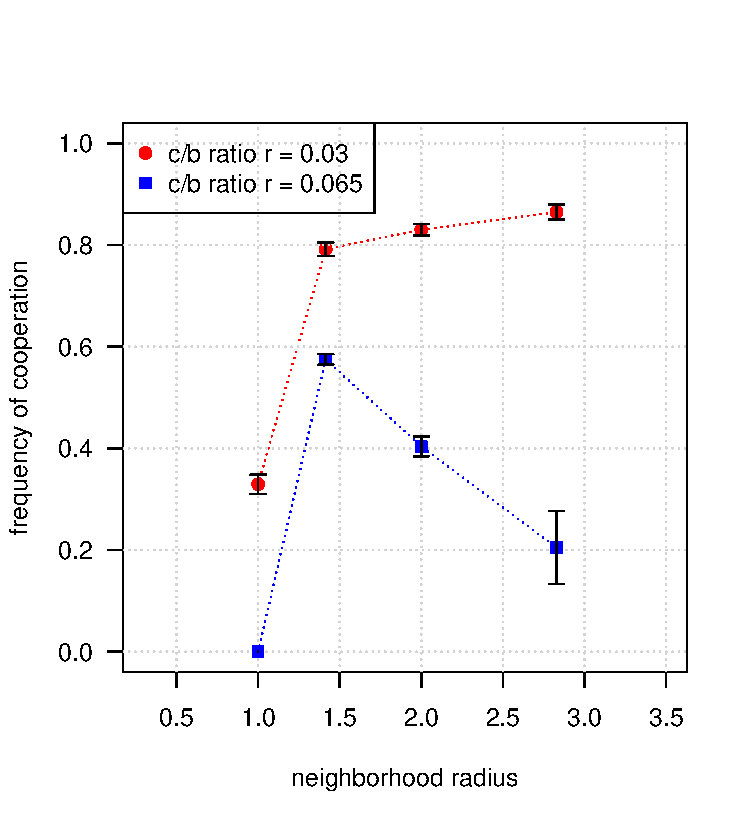
\includegraphics[width=9.5cm]{task2_radiusplot}
	\caption{Spatial PD game simulations with fixed cost-benefit-ratio and different neighborhood sizes. Radius 1 is adequate to 4 neighbors, radius 1.4 = 8 neighbors, radius 2 = 12 neighbors and radius 2.8 = 24 neighbors.  \textbf{[ t = 10000, i = 10 ]} }\label{fig: task2_radiusplot}
\end{figure}


\subsection{Effect of mixed strategies}

In our third experiment, we compared the effect of spatial structure in the mixed-strategy HD game with that in the pure-strategy game.


\begin{figure}[H]
	\centering 
	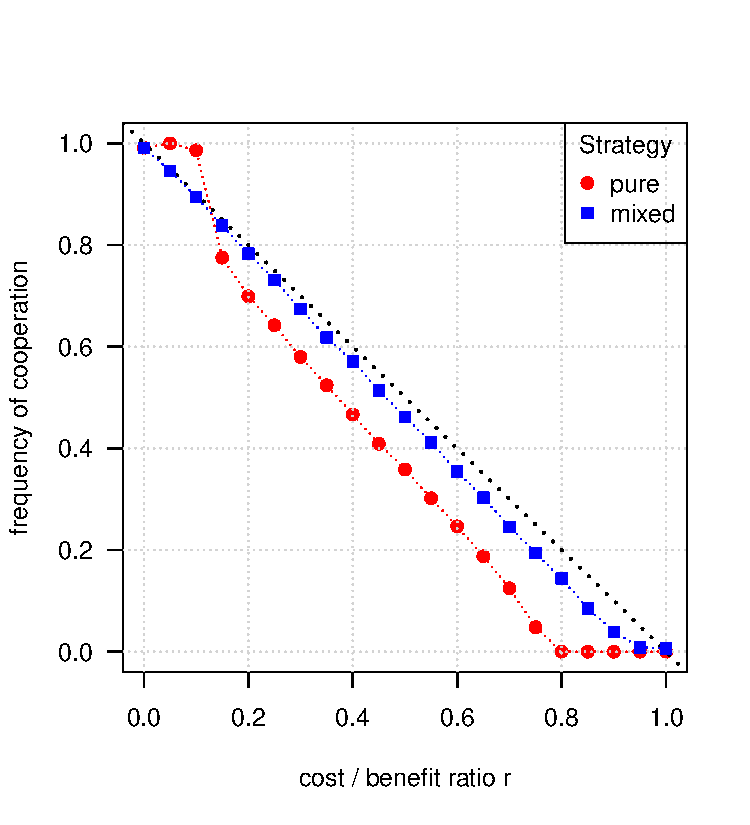
\includegraphics[width=9.5cm]{task3_multiplot}
	\caption{Spatial HD game simulations with neighborhood size 8 and different strategies. The dotted black line depicts the frequency of cooperation in nonspatial games.  \textbf{[ t = 10000, i = 10 ]} }\label{fig: task3_multiplot}
\end{figure}





